%%%%%%%%%%%%%%%%%%%%%%%%%
% DISTANCE TO CENTROIDS %
%%%%%%%%%%%%%%%%%%%%%%%%%

% \section{Distance to Centroids}
% from the LOD paper

%%%%%%%%%%%
% RESULTS %
%%%%%%%%%%%

\section{Experimental Results and Discussion}

We now present and discuss the results for CIFAR-10/ViT and MNIST/CNN. Both dataset/architecture pairs show similar trends in our analysis of the results. For context, in the case of MNIST with 60,000 well-balanced training examples (each digit class has approximately 6,000 examples), we find 54 occurrences of 8's misclassified as 9's. We note that 0's are the least likely and 8's are the most likely digits to be misclassified. Other digits that are less likely to be misclassified are 1's, 6's and 5's. Digit 8 is likely to be misclassified as a 6 or 9, while digit 3 is likely to be misclassified as a 2, 5 or 9. One can see how, already by itself, this kind of analysis can offer some insight onto the behaviour of specific outputs in relation to other outputs and our confidence in the results, differently from the overall headline classification accuracy figure that in the case of MNIST has been close to $99\%$ accuracy. 

%The confusion matrix shown in Figure \ref{fig:mnist_training_confusion_matrix} provides some insights into what the most likely MNIST misclassifications are. The training dataset contains 60,000 images and is well-balanced (each digit class has approximately 6,000 examples). On the diagonal we see the number of correct classifications and off-diagonal we see the pair-wise incorrect classifications e.g. there are 54 occurrences of 8 misclassified as a 9. We note that number zero is the digit less likely (sum of the row values minus the diagonal is the smallest), and number eight is the digit most likely to be misclassified  (sum of the row values minus the diagonal is the greatest). Other digits that are less likely to be misclassified are digits one, six and five. Digit eight is likely to be misclassified as six or nine, while digit three is likely to be misclassified as two, five or nine.

\textbf{Clustering}: We observe that calculating the average softmax outputs for all the correct classifications provides a good initialization for the K-means algorithm centroids. Clustering converges quickly and assigns all but two of the approximately 59,000 correctly classified examples (in the case of MNIST/CNN) to the correct class centroids. For example, all digits 0 are assigned to the same cluster that we shall label \textit{cluster 0}. In this case, we say that the unsupervised clustering task presents \emph{high fidelity} to the supervised classification task, and in this case it acts as a good proxy for assessing confidence in its predictions.%, the correlation between cluster assignments and true labels providing independent validation. 

We compute all pairwise distances between the 10-class centroids in the softmax space.\footnote{($\binom{10}{2}=45$ pairs; although this may be a computationally costly task with an increasing number of classes, we note that typically the number of classes is much smaller than the number of parameters and the data set.} The distances exhibit $d_{min}=1.368$, $d_{max}=1.402$, $\mu=1.389$ and $\sigma=0.009$. These values approach $\sqrt{2}$, the maximum distance between points in the probability-constrained simplex, indicating that the model distributes classes at near-maximal separation in the output space. The supervised learning task achieved this separation through gradient descent on the cross-entropy loss; the unsupervised learning task confirms what has been induced by the classification task given the high-fidelity of the results.

The above combination of supervised and unsupervised learning allows us to examine edge cases, where images are correctly classified but incorrectly clustered. The goal is to understand the softmax output better in connection with the distances to class centroids. Figure \ref{fig:ImageID8688_Softmax_Clustering} shows a correctly classified 6 that is incorrectly clustered as a 5, where the softmax outputs for digits 5 and 6 are very close (0.491 and 0.495, respectively), and the distances of that example to the centroid of clusters 5 and 6 are also very close (0.696 and 0.697, respectively). %Therefore, the softmax output is marginally higher for digit six, while the softmax output is marginally closer to the class 5 centroid. 
The softmax output shows high entropy, while the distances to class centroids show an example that is about 1.2 units away from all class centroids and close to 0.7 from both centroids 5 and 6. This illustrates a case where the model exhibits uncertainty, as would be expected from the softmax histogram already, but there are clear differences to the clustering histogram, despite the high-fidelity, to be investigated.

%between two plausible classes, positioning the output almost equidistant between their centroids in the probability simplex. The slight discordance between classification and clustering in this case reveals a boundary condition in the model's decision space.

\begin{figure}[ht]
    \centering
    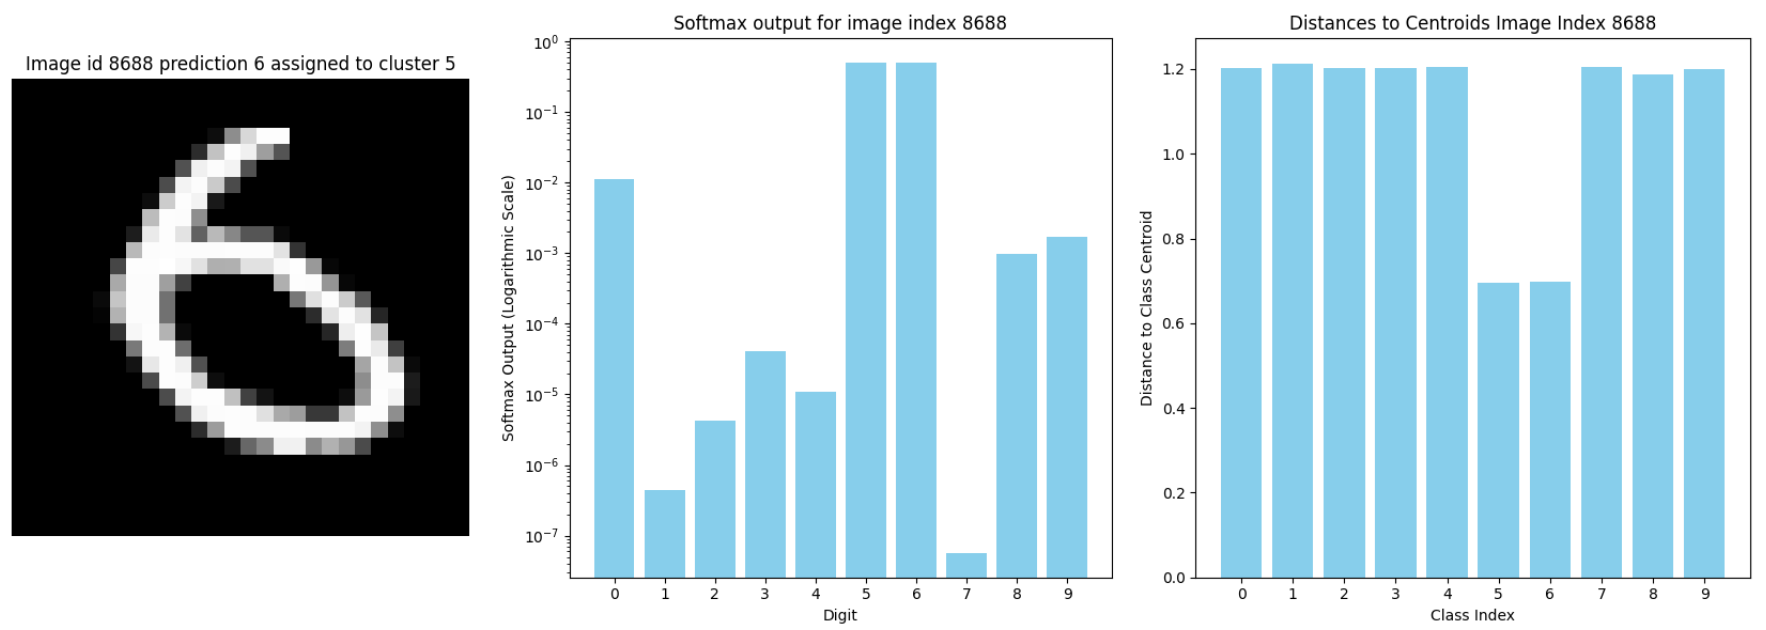
\includegraphics[width=0.99\columnwidth]{Figures/Results/ImageID8688_Softmax_Clustering.png}
    \caption{Left to right, MNIST Training Data Image ID 8688 digit 6, the network softmax output and the distances to class centroids, correctly classified as 6 and incorrectly clustered as 5. Notice that the y axis is not on logarithmic scale in this case.     %MNIST_TRAINING_DATASET_ACC_RATIO_VS_THRESHOLD
    }
\label{fig:ImageID8688_Softmax_Clustering}
\end{figure}

\begin{figure}[ht!]
    \centering
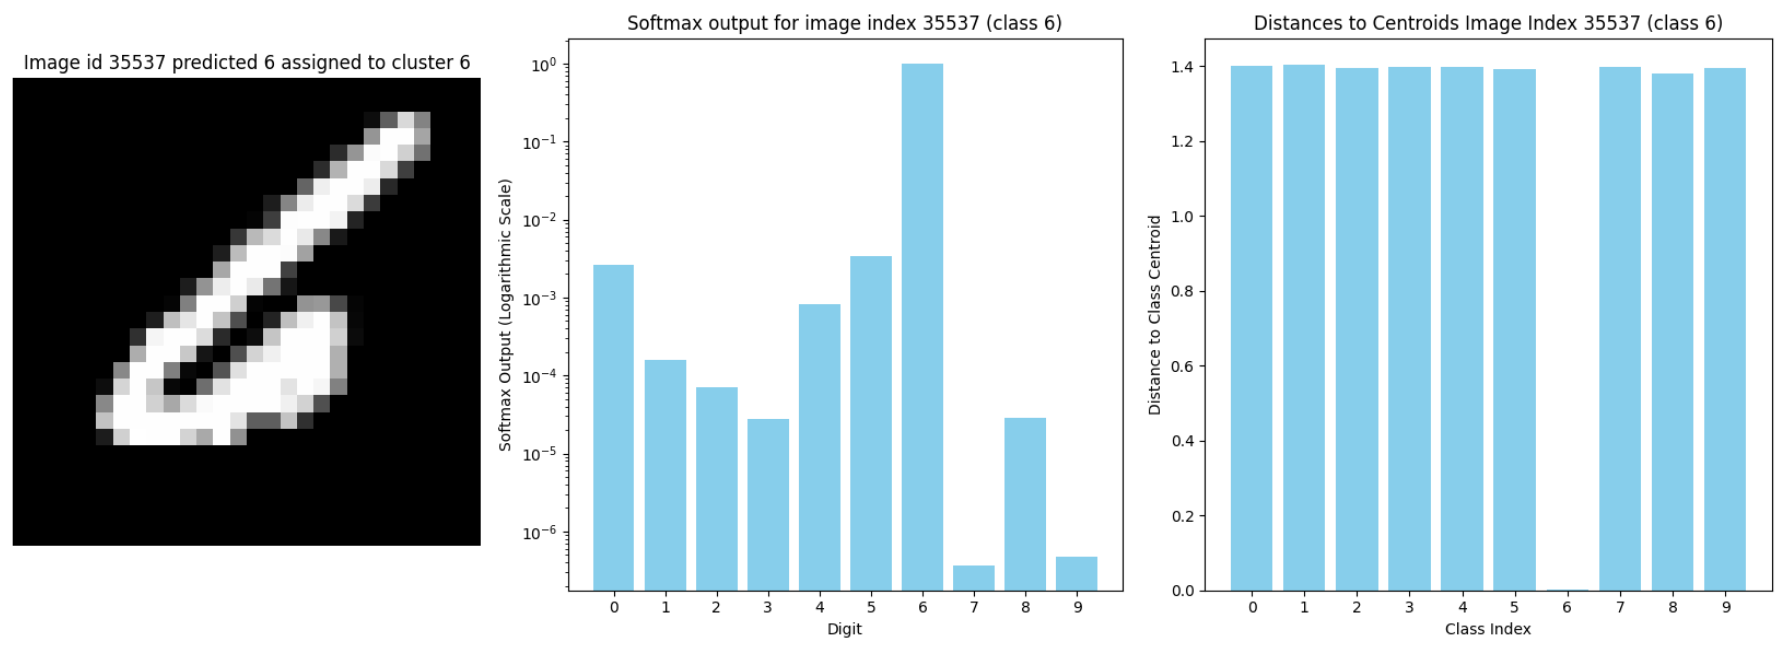
\includegraphics[width=0.99\columnwidth]{Figures/Results/ImageID35537_Softmax_Clustering.png}
    \caption{Left to right, MNIST Training Data Image ID 35537 digit 6, the network softmax output and the distances to class centroids, correctly classified and correctly clustered as 6.     %MNIST_TRAINING_DATASET_ACC_RATIO_VS_THRESHOLD
    }
\label{fig:ImageID35537_Softmax_Clustering}
\end{figure}

The next example presents a contrasting case to the previous edge case. Figure \ref{fig:ImageID35537_Softmax_Clustering} shows a 6 where the softmax output assigns 0.993 probability to class 6, with all other classes receiving probabilities below 0.004 (the y axis is in log scale). The low entropy of the softmax output matches a clear separation of centroid distances. As before, there are differences in the histograms to be further investigated. 

In what follows, more than investigating individual examples case-by-case as in Figures \ref{fig:ImageID8688_Softmax_Clustering} and \ref{fig:ImageID35537_Softmax_Clustering}, we will use the clustering (and hence the differences in the histograms) to seek to identify general trends for entire classes represented by the cluster centroids.

\textbf{Varying Thresholds}: The uncertainty that the above edge case exemplifies suggests that it would be reasonable to classify the data point, not as a 6 or a 5, but as \textit{unknown}. In fact, it could be argued that in this case the classification should be ``5 or 6", in that the image is likely to be of one of those two digits, but it is not known which. We now investigate, by varying the threshold used to define cluster membership, how certain examples may fall into an \textit{unknown} region of the clustering. We evaluate how accuracy varies by changing this threshold and also how many examples fall into the \textit{unknown} region (retention), as well as the ratios of correct to incorrect predictions. 

Figure~\ref{fig:MNIST_TRAINING_DATASET_ACC_RATIO_VS_THRESHOLD} depict test set accuracy, retention (the percentage of examples belonging to the cluster hypersphere) and correct-to-incorrect ratio versus threshold (distance to predicted class centroid) for CIFAR/ViT (top) and MNIST/CNN (bottom). The y-left axis (percentage) ranges from 98.0\% to 100.0\% for both. For CIFAR/ViT, retention (blue) decreases from 100.0\% to 98.0\%, accuracy (green) increases from 99.4\% to 99.7\%, and the ratio (red) rises from 197:1 to 536:1 as the threshold decreases from 0.80 to 0.05. For MNIST/CNN, retention decreases from 100.0\% to 92.0\%, accuracy increases from 98.0\% to 99.0\%, and the ratio rises from 64:1 to 632:1 over the same threshold range. The ViT created more compact clusters, noting the ViT has 2 orders of magnitude more parameters than the CNN.

%The ViT/CIFAR-10 plot shows a tighter clustering on the y-left axis, with retention and accuracy varying within a 2.0\% range, compared to a 8.0\% range for CNN/MNIST, indicating the ViT architecture created more compact clusters, noting the ViT has 2 orders of magnitude more parameters than the CNN architecture.

\begin{figure}[ht!]
    \centering
    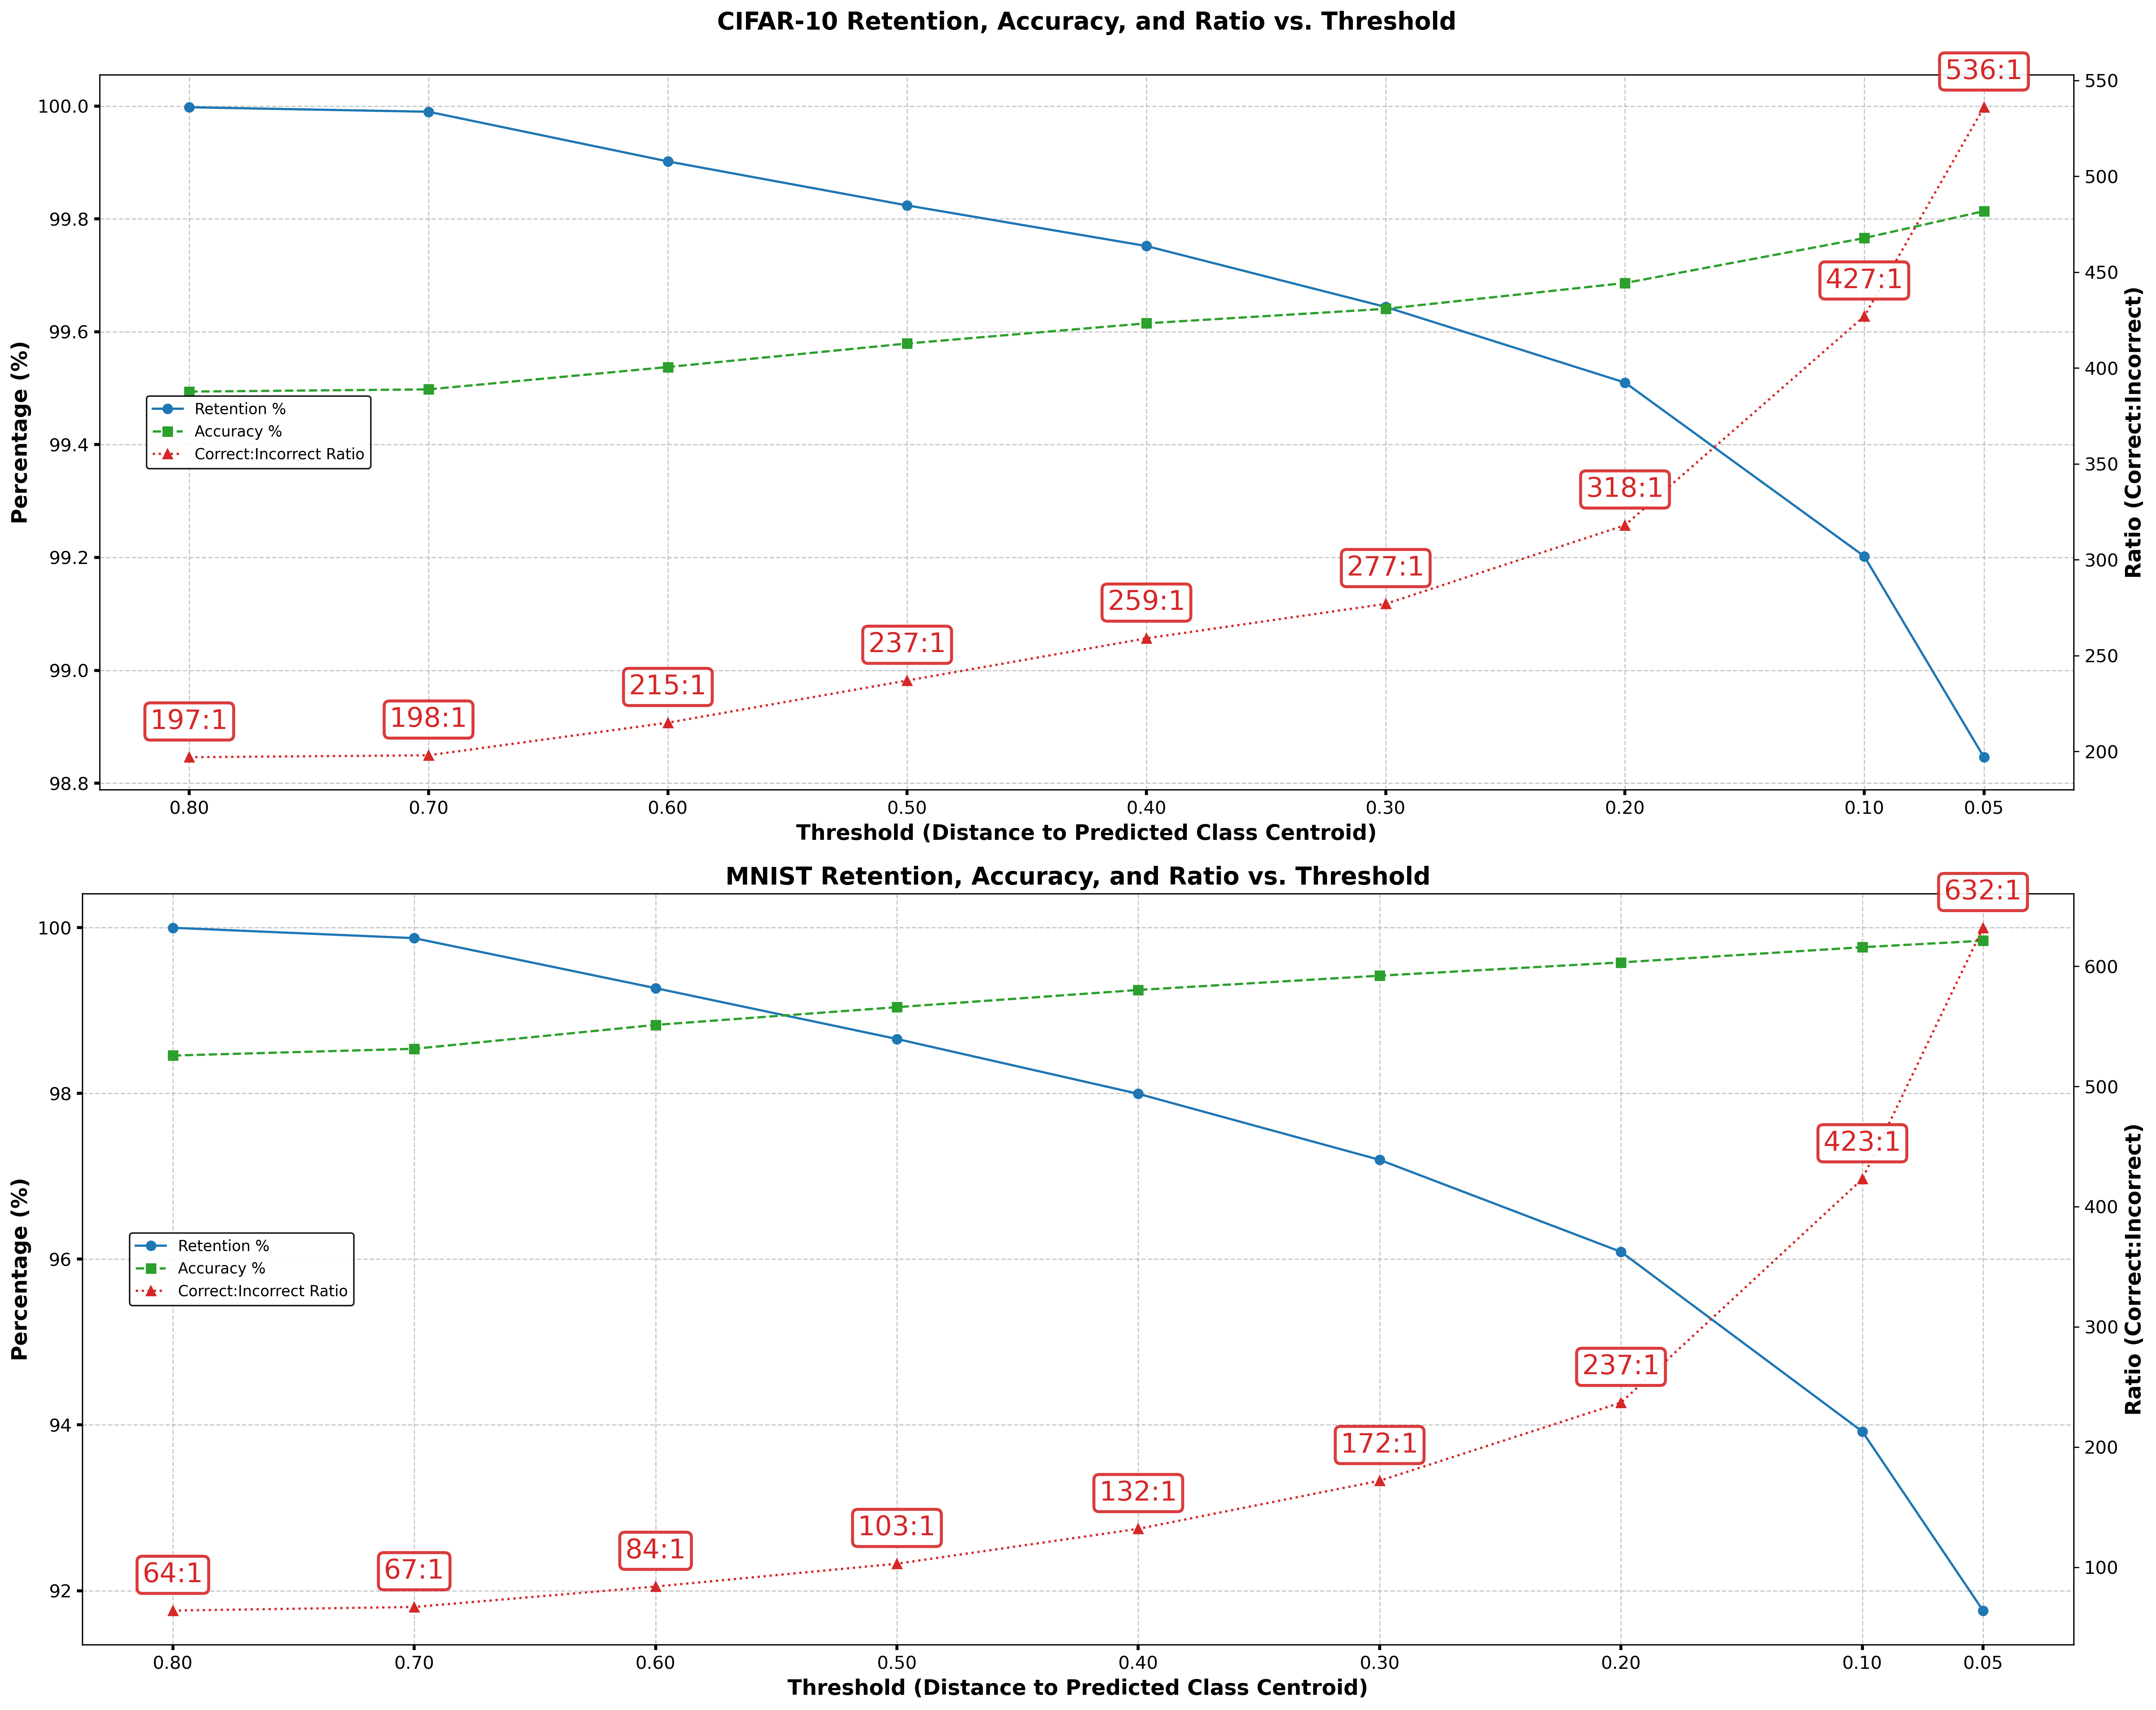
\includegraphics[width=0.99\columnwidth]{Figures/Results/cifar10_mnist_retention_accuracy_ratio_vs_threshold.png}
    \caption{Retention, accuracy and correct-incorrect ratio vs Threshold ViT trained on CIFAR-10 and CNN trained on MNIST where the training dataset results are shown. The red plot represents the ratio of correct to incorrect predictions across all classes at given thresholds e.g. for CNN/MNIST at threshold 0.8 the ratio is 64:1, at threshold 0.05 the ratio is 632:1. The green plot is accuracy at every threshold e.g. at threshold 0.8 the accuracy is approximately 98.5\%, 64/(64+1), and at threshold 0.05 the accuracy is approximately 100\%, 632/(632+1). The blue plot represents the percentage of correct predictions that are being discarded as the threshold decreases e.g. at threshold 0.8 all correct predictions are kept while at threshold 0.05 over 8\% of the correct predictions are discarded i.e. classed as \textit{unknown}.}
\label{fig:MNIST_TRAINING_DATASET_ACC_RATIO_VS_THRESHOLD}
\end{figure}


% Plot created manually from MNIST and CIFAR10 plots created by function plot_accuracy_vs_distance_linear_fit
% Take 2
% repo: git@github.com:dsikar/IJCNN-2025.git
% file: scripts/hypersphere.py
% commit 06ce13ff908c33417afd27f4ad1fb9cb398bebd9
% TODOS
% 1. remove green accuracy labels
% 2. Improve caption
% 3. Create CIFAR-10 plot


%%%%%%%%%%%%%%%%%%%%%%%%%%%%%%%%%%%%%%%%%
% MISCLASSIFIED CHARACTERS MIN AND AVGS %
%%%%%%%%%%%%%%%%%%%%%%%%%%%%%%%%%%%%%%%%%

\textbf{Out-of-distribution Data:} Predictions for in-distribution data are expected to fall closer to class centroids, and predictions for out-of-distribution data further away. To study out-of-distribution data predictions we \textit{MNISTify} the English Handwritten Characters dataset \cite{deCampos09} (separating digits from alphabetic characters for the sake of analysis), and the CIFAR-10 dataset. %by adapting the number of channels and ratio to conform to our CNN architecture. 
Figure \ref{fig:closest_alphabetic_characters_to_each_digit} shows which characters are nearest to each MNIST/CNN digit class centroid and also the average distance from the given class centroid (observing upper and lower case). For example, the lower case \textit{z} character shown (third from left) is among all alphabetic characters the nearest to centroid of digit class 2 (0.00893), where the average lower case \textit{z} is 0.20964 distance units away. Characters lower case \textit{b}, upper case \textit{B} and lower case \textit{a} show strong resemblance to digits \textit{6}, \textit{8} and \textit{9}, respectively. This is reflected is the clustering of the alphabetic dataset. Notice that no further training or fine-tuning of the CNN took place here. We only used MNIST/CNN for inference given the new character data set. We are interested in identifying, in the case of out-of-distribution data, how reasonable a prediction may be on average (not individual cases), as in the case of lower case \textit{z} above, and which predictions should fall in the \textit{unknown} region. 

\begin{figure}[ht!]
    \centering
    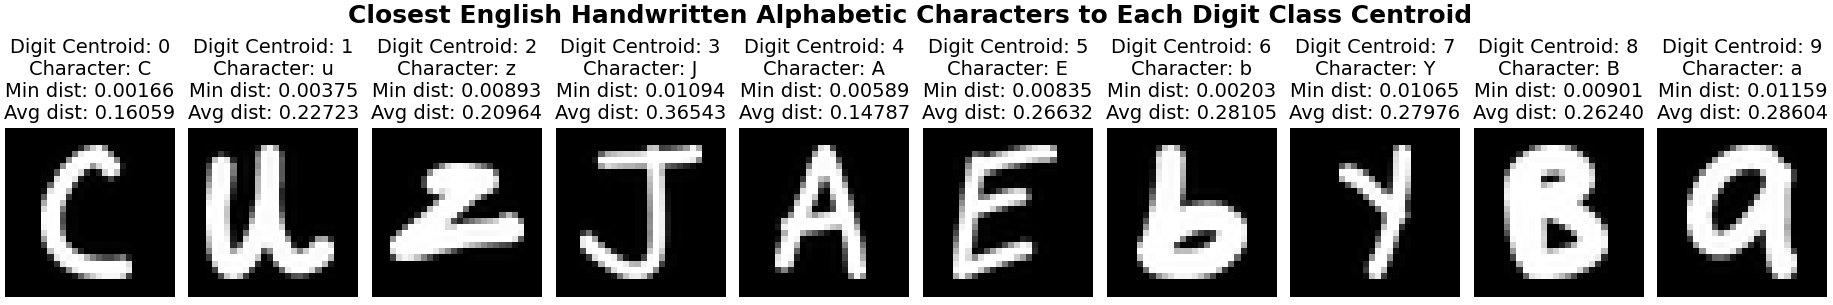
\includegraphics[width=0.99\columnwidth]{Figures/Results/closest_alphabetic_characters_to_each_digit.png}
    \caption{English Handwritten Alphabetic Characters nearest distance and example, and averages}
\label{fig:closest_alphabetic_characters_to_each_digit}
\end{figure}

%%%%%%%%%%%%%%%%%%%%%%%%%%%%%%%
% MNISTified CIFAR10 EXAMPLES %
%%%%%%%%%%%%%%%%%%%%%%%%%%%%%%%
% removed for lack of space
% Figure \ref{fig:english_handwritten_characters_alphabetic_softmax_averages} shows examples of the \textit{MNISTified} CIFAR-10 dataset. As expected, the examples bear no resemblance to digits, which as we shall see is reflected in the clustering. In this case, one would expect all examples to be classified as \textit{unknown}.

% % plot_mnistified_samples(train_ds, cifar10_classes, convert_cifar10_to_mnist_format, filename='figures/mnistified_cifar10.png', save_flag=True)
% \begin{figure*}[ht!]
%     \centering
%     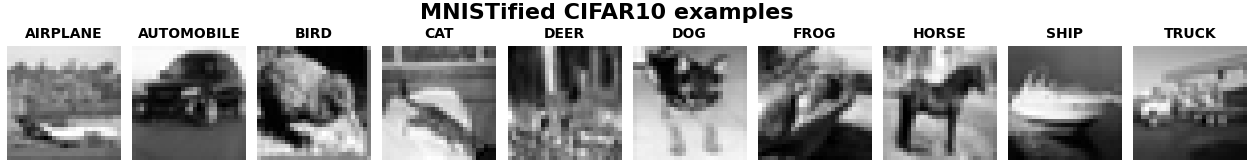
\includegraphics[width=0.99\textwidth]{Figures/ThresholdAnalysis/mnistified_cifar10.png}
%     \caption{MNISTified CIFAR10 Dataset Examples}
% \label{fig:english_handwritten_characters_alphabetic_softmax_averages}
% \end{figure*}

Table~\ref{tab:threshold_percentages} shows dataset percentages that fall bellow or at/above threshold with varying thresholds. For example, for threshold 0.8, all datasets except \textit{MNISTified} CIFAR-10 have 100\% of the examples below threshold. At the lowest threshold of 0.05, CIFAR-10 has the highest percentage of examples below threshold, indicating the tightest clustering, followed by MNIST, where the number of in-cluster examples starts dropping significantly at 0.3 threshold. The \textit{MNISTified} English Handwritten Digits are more tightly clustered than the English Alphabetical Characters, as the former bears a closer resemblance to the MNIST dataset, and the latter have no equivalent labels in the MNIST dataset and consequently all predictions are technically incorrect. Notice that for the \textit{MNISTified} CIFAR-10, another case of all predictions being incorrect by default, and bearing no resemblance whatsoever to digits, has 97\% of examples rejected (excluded from all the clusters) at a threshold of 0.05. %The implication is there exist examples that bear no resemblance to digits, still classified by the neural network with a high degree of confidence, however, centroid proximity does increase the likelihood that the prediction is correct for in-distribution data.

\begin{table}[ht]
\centering
\scriptsize
\caption{Percentage of examples below and at or above thresholds for distance to predicted class centroid across five datasets. Total examples: CIFAR-10 (50,000), MNIST (60,000), MNISTified English Handwritten Digits (550), MNISTified English Handwritten Alphabetical Characters (2,860), MNISTified CIFAR-10 (50,000).}
\label{tab:threshold_percentages}
\begin{tabular*}{\textwidth}{@{\extracolsep{\fill}} c *{10}{S[table-format=3.1]}}
\toprule
 & \multicolumn{2}{c}{CIFAR-10} & \multicolumn{2}{c}{MNIST} & \multicolumn{2}{c}{Eng. Digits} & \multicolumn{2}{c}{Eng. Alphabetical} & \multicolumn{2}{c}{MNISTified CIFAR-10} \\
\cmidrule(lr){2-3} \cmidrule(lr){4-5} \cmidrule(lr){6-7} \cmidrule(lr){8-9} \cmidrule(lr){10-11}
Threshold & {Below} & {At/Above} & {Below} & {At/Above} & {Below} & {At/Above} & {Below} & {At/Above} & {Below} & {At/Above} \\
\midrule
0.8  & 100.0 & 0.0  & 100.0 & 0.0  & 100.0 & 0.0  & 100.0 & 0.0  & 98.2  & 1.8  \\
0.7  & 100.0 & 0.0  & 99.9  & 0.1  & 99.3  & 0.7  & 97.4  & 2.6  & 85.5  & 14.5 \\
0.6  & 99.9  & 0.1  & 99.3  & 0.7  & 96.5  & 3.5  & 90.2  & 9.8  & 67.4  & 32.6 \\
0.5  & 99.8  & 0.2  & 98.7  & 1.3  & 93.1  & 6.9  & 83.0  & 17.0 & 52.6  & 47.4 \\
0.4  & 99.8  & 0.2  & 98.0  & 2.0  & 89.3  & 10.7 & 75.0  & 25.0 & 39.1  & 60.9 \\
0.3  & 99.6  & 0.4  & 97.2  & 2.8  & 86.0  & 14.0 & 67.2  & 32.8 & 27.2  & 72.8 \\
0.2  & 99.5  & 0.5  & 96.1  & 3.9  & 81.6  & 18.4 & 58.0  & 42.0 & 16.5  & 83.5 \\
0.1  & 99.2  & 0.8  & 93.9  & 6.1  & 72.4  & 27.6 & 47.0  & 53.0 & 6.9   & 93.1 \\
0.05 & 98.8  & 1.2  & 91.8  & 8.2  & 67.8  & 32.2 & 38.7  & 61.3 & 3.0   & 97.0 \\
\bottomrule
\end{tabular*}
\end{table}

Figure~\ref{fig:Exclusion_Rate_vs_Threshold} shows the relationship between distance thresholds (x-axis) and exclusion percentages (y-axis). Five datasets are represented: CIFAR-10 (blue), MNIST (green), MNISTified English Digits (purple), MNISTified English Alphabetical (red), and MNISTified CIFAR-10 (yellow), with dataset counts indicated in parentheses. The x-axis ranges from 0.80 to 0.05, representing decreasing threshold values for the distance to predicted class centroid. The y-axis shows percentage values from 0\% to 100\%. MNISTified CIFAR-10 exhibits the highest exclusion rates across all thresholds. The MNISTified English Alphabetical dataset shows moderate exclusion rates (up to 61\%), while MNISTified English Digits demonstrates lower exclusion rates (up to 32\%). Both MNIST and CIFAR-10 maintain minimal exclusion rates below 10\% across all thresholds, with CIFAR-10 showing the lowest values overall, remaining under 1\%. 

\begin{figure}[ht!]
    \centering
    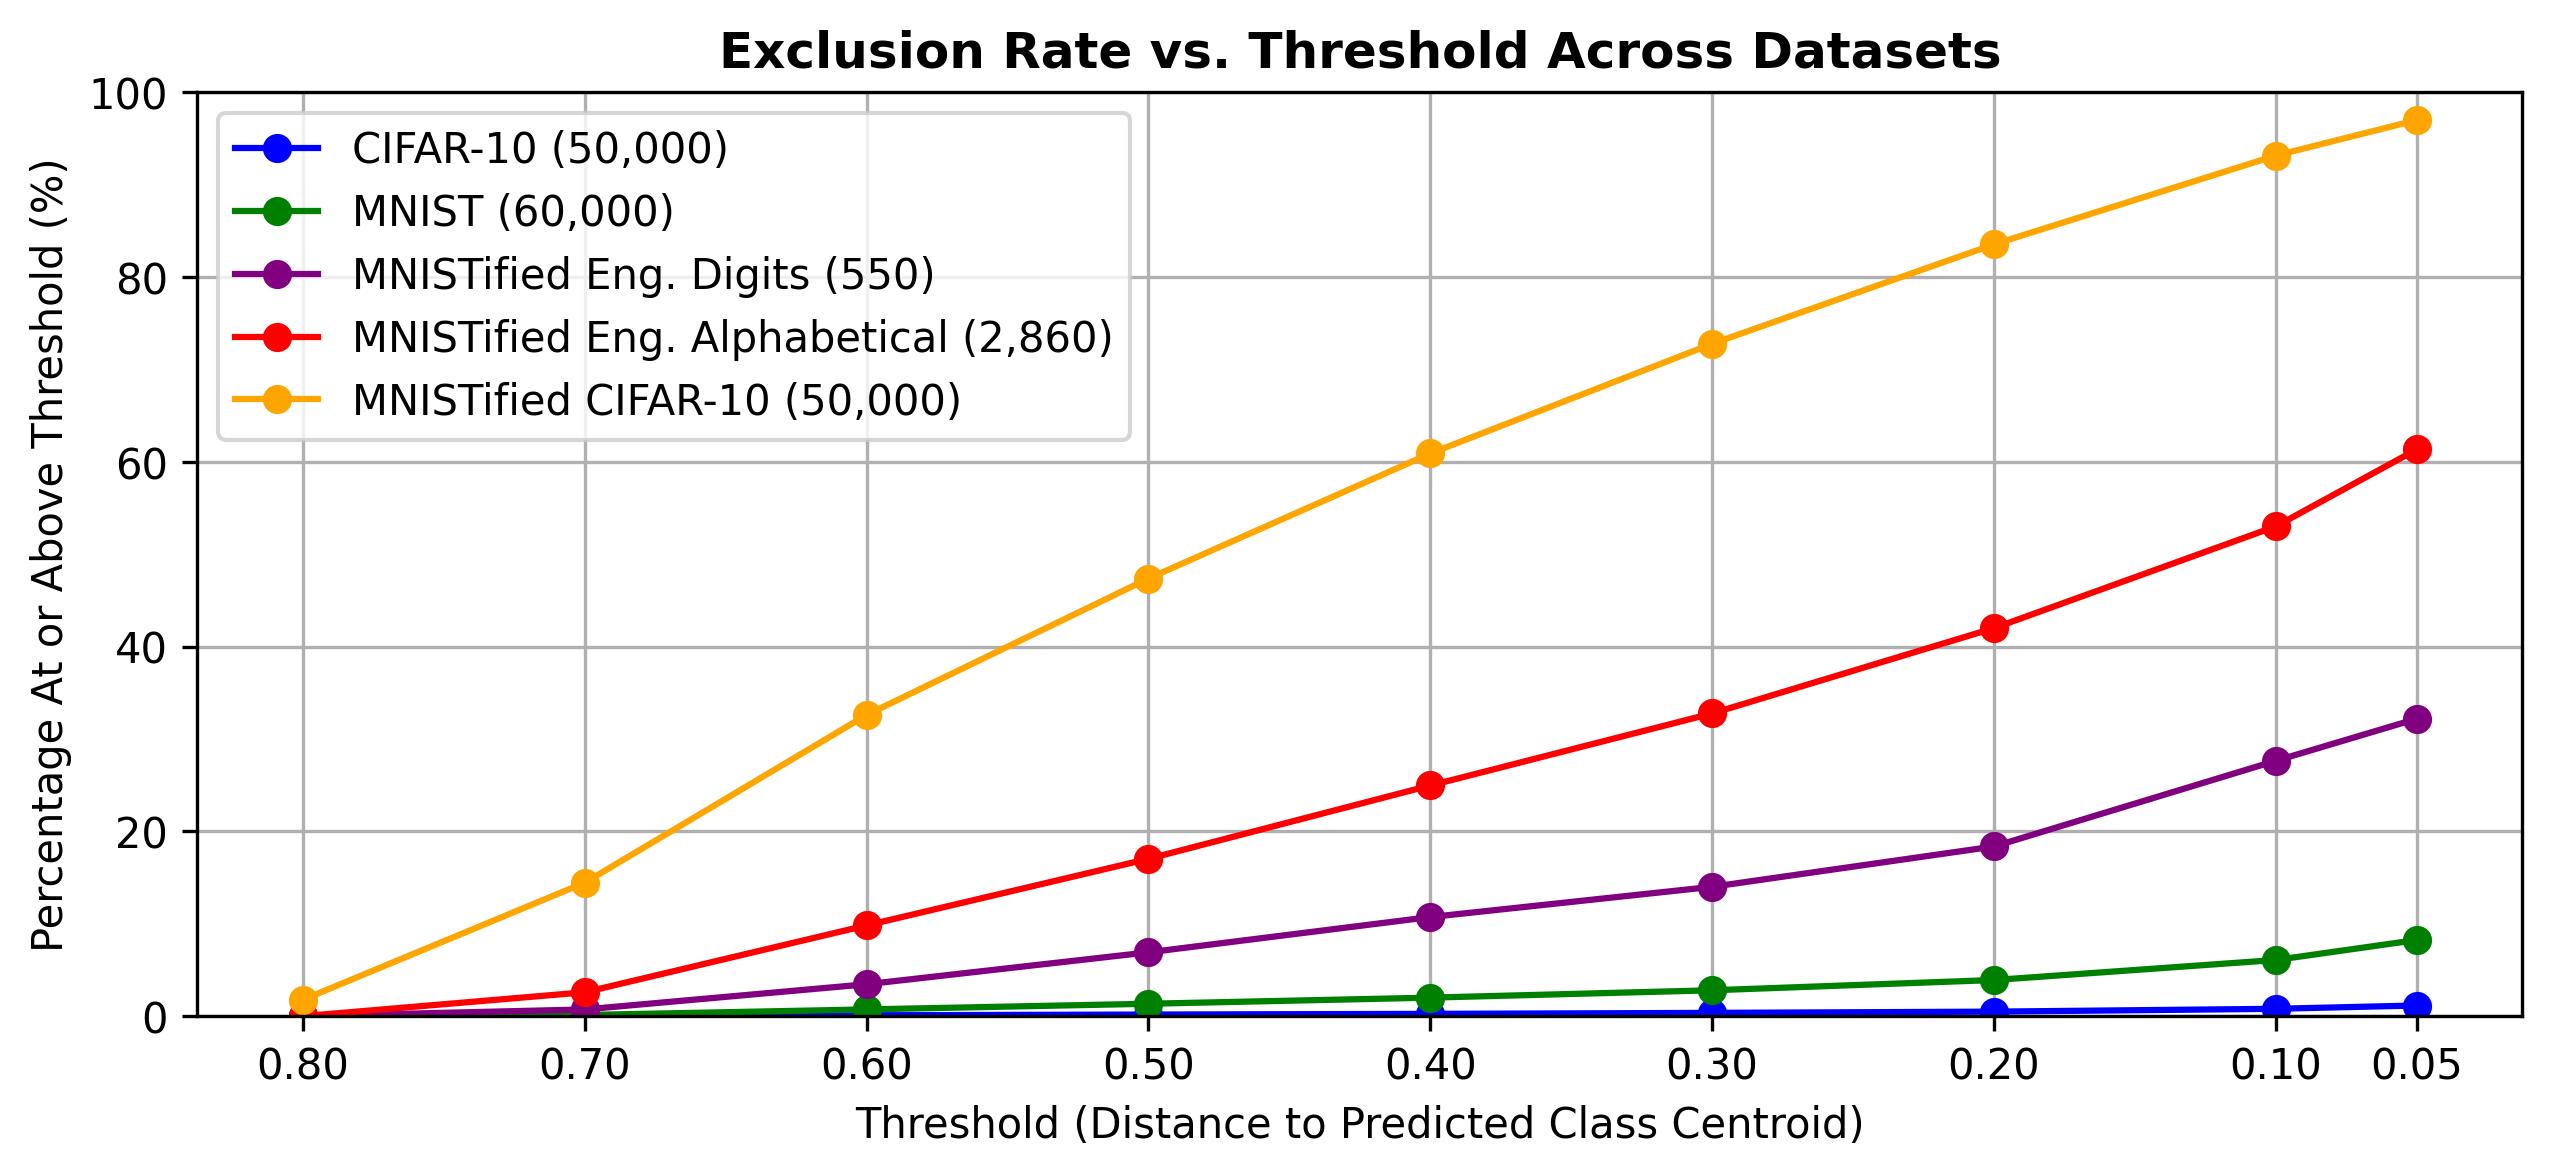
\includegraphics[width=0.99\columnwidth]{Figures/Results/Exclusion_Rate_vs_Threshold.png}
    \caption{Percentage of examples at or above thresholds for distance to predicted class centroid across five datasets, showing higher exclusion rates for English Alphabetical Characters and MNISTified CIFAR-10. Total examples: CIFAR-10 (50,000), MNIST (60,000), Eng. Digits (550), Eng. Alphabetical (2,860), MNISTified CIFAR-10 (50,000).}
\label{fig:Exclusion_Rate_vs_Threshold}
\end{figure}

\begin{table}[ht]
\centering
%\small
\scriptsize
\caption{Density of points (\(N_k\), \(\rho_k\)) in 10-dimensional spherical shells and inner sphere, based on distance to predicted class centroid. Higher densities in outer shells for English Alphabetical Characters and MNISTified CIFAR-10 indicates greater exclusion. Total examples: CIFAR-10 (50,000), MNIST (60,000), Eng. Digits (550), Eng. Alphabetical (2,860), MNISTified CIFAR-10 (50,000).}
\label{tab:density}
\begin{tabular}{@{} l l S[table-format=1.5e-1] *{5}{cc} @{}}
\toprule
 & & & \multicolumn{2}{c}{CIFAR-10} & \multicolumn{2}{c}{MNIST} & \multicolumn{2}{c}{Eng. Digits} & \multicolumn{2}{c}{Eng. Alphabetical} & \multicolumn{2}{c}{M'fied CIFAR-10} \\
\cmidrule(lr){4-5} \cmidrule(lr){6-7} \cmidrule(lr){8-9} \cmidrule(lr){10-11} \cmidrule(lr){12-13}
{Shell} & {Radii} & {Volume} & {$N_k$} & {$\rho_k$} & {$N_k$} & {$\rho_k$} & {$N_k$} & {$\rho_k$} & {$N_k$} & {$\rho_k$} & {$N_k$} & {$\rho_k$} \\
\midrule
1 & 0.7--0.8 & 2.01786e-1 & 4 & 2.0e1 & 75 & 3.7e2 & 4 & 2.0e1 & 74 & 3.7e2 & 6336 & 3.1e4 \\
2 & 0.6--0.7 & 5.6616e-2 & 44 & 7.8e2 & 362 & 6.4e3 & 15 & 2.6e2 & 207 & 3.7e3 & 9077 & 1.6e5 \\
3 & 0.5--0.6 & 1.29295e-2 & 39 & 3.0e3 & 368 & 2.8e4 & 19 & 1.5e3 & 206 & 1.6e4 & 7379 & 5.7e5 \\
4 & 0.4--0.5 & 2.22299e-3 & 36 & 1.6e4 & 397 & 1.8e5 & 21 & 9.4e3 & 227 & 1.0e5 & 6767 & 3.0e6 \\
5 & 0.3--0.4 & 2.52346e-4 & 54 & 2.1e5 & 478 & 1.9e6 & 18 & 7.1e4 & 223 & 8.8e5 & 5934 & 2.4e7 \\
6 & 0.2--0.3 & 1.47973e-5 & 67 & 4.5e6 & 666 & 4.5e7 & 24 & 1.6e6 & 264 & 1.8e7 & 5383 & 3.6e8 \\
7 & 0.1--0.2 & 2.60882e-7 & 154 & 5.9e8 & 1301 & 5.0e9 & 51 & 2.0e8 & 315 & 1.2e9 & 4802 & 1.8e10 \\
8 & 0.05--0.1 & 2.54767e-10 & 178 & 7.0e11 & 1296 & 5.1e12 & 25 & 9.8e10 & 238 & 9.3e11 & 1919 & 7.5e12 \\
Inner & $\leq$0.05 & 2.49039e-13 & 49423 & 2.0e17 & 55056 & 2.2e17 & 373 & 1.5e15 & 1106 & 4.4e15 & 1513 & 6.1e15 \\
\bottomrule
\end{tabular}
\end{table}


% scripts/color-coded-rings.py
\begin{figure}[ht]
    \centering
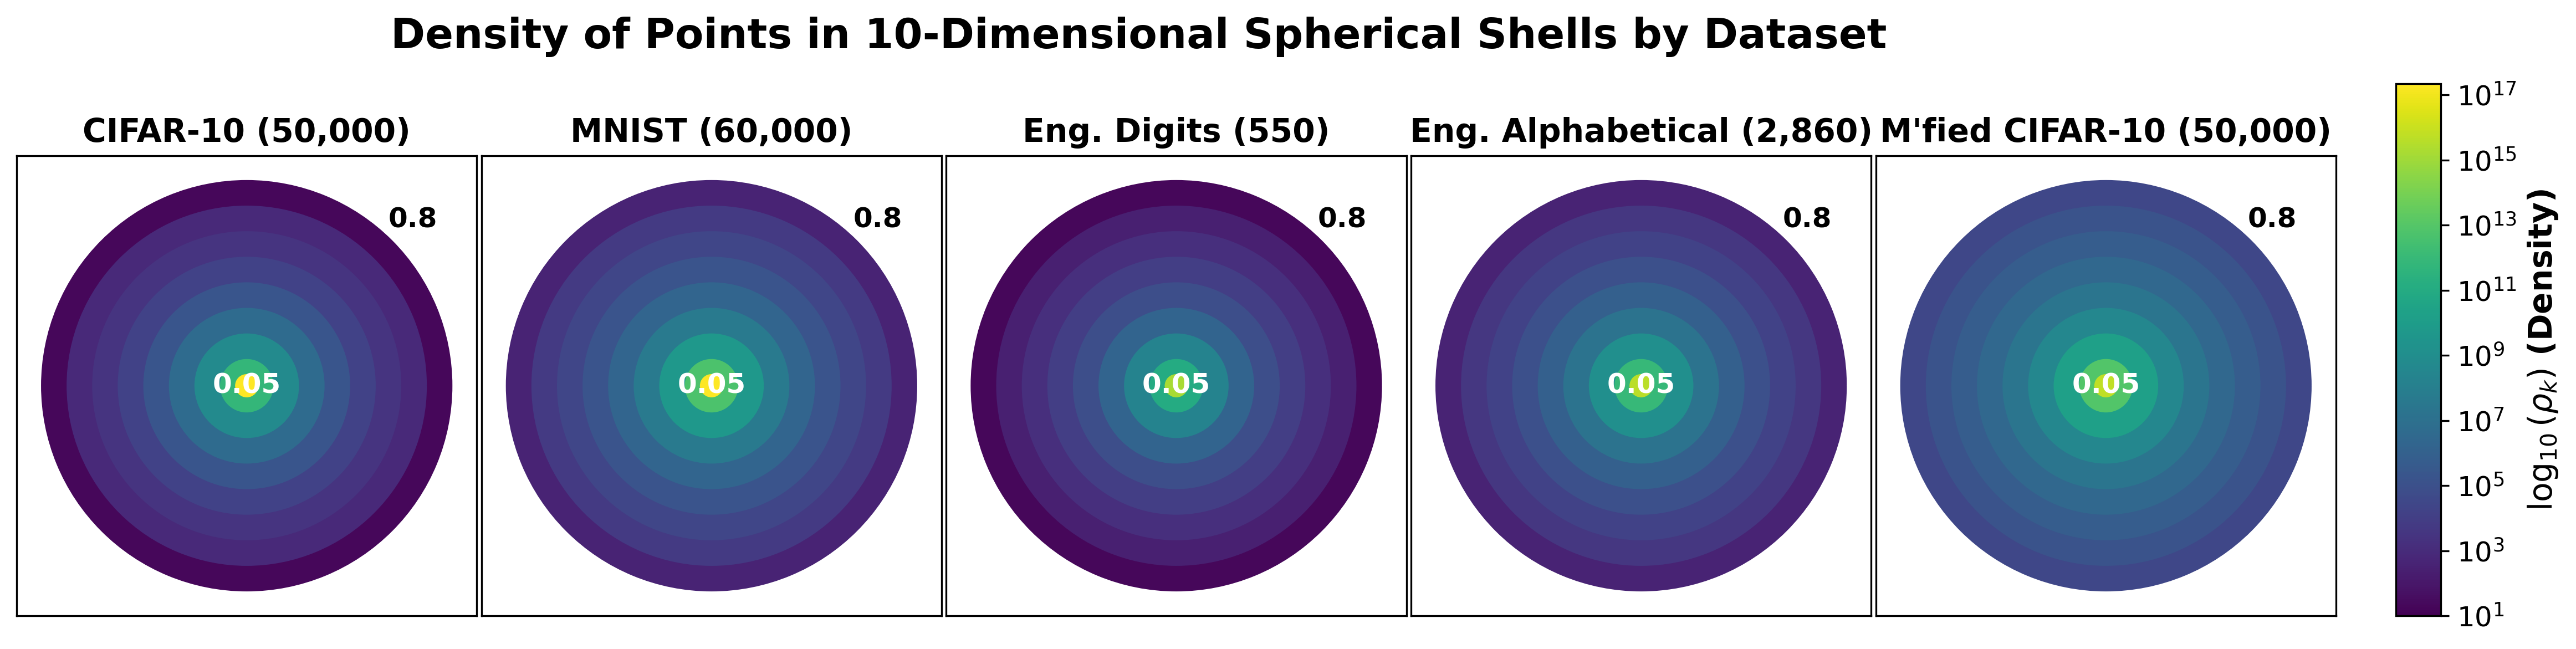
\includegraphics[width=0.99\columnwidth]{Figures/Results/density_rings.png}
\caption{Density of points in 10-dimensional spherical shells, visualized as concentric rings. Color intensity represents $\log_{10}(\rho_k)$, with brighter colors indicating higher density. English Alphabetical Characters and MNISTified CIFAR-10 show higher density in outer shells, reflecting greater exclusion. Total examples: CIFAR-10 (50,000), MNIST (60,000), Eng. Digits (550), Eng. Alphabetical (2,860), MNISTified CIFAR-10 (50,000).}
\label{fig:density_rings}
\end{figure}

\textbf{Cluster Density}: Figure~\ref{fig:density_rings} presents a concentric ring visualization of the density of points (\(\rho_k\)) in 10-dimensional spherical shells, defined by distance thresholds to the predicted class centroid [0.7--0.8, 0.6--0.7, 0.5--0.6, 0.4--0.5, 0.3--0.4, 0.2--0.3, 0.1--0.2, 0.05--0.1] and an inner sphere (\(\leq 0.05\)), across five datasets: CIFAR-10 (50,000 examples), MNIST (60,000 examples), English Handwritten Digits (550 examples), English Handwritten Alphabetical Characters (2,860 examples), and MNISTified CIFAR-10 (50,000 examples). The figure, a row of 5 subplots with a shared colorbar, encodes the density of softmax outputs in the 10-dimensional probability simplex, highlighting the higher exclusion rates (larger distances) for English Alphabetical Characters and MNISTified CIFAR-10. Next we examine the figure’s design, interpret its density patterns, and address the implications and limitations of projecting high-dimensional data into a 2D representation: each subplot represents a dataset, with eight concentric annuli corresponding to the shells and a central circle for the inner sphere. The radii are scaled to the thresholds (0.8 to 0.05), ensuring the outermost shell (0.7--0.8) is wider than the innermost (0.05--0.1), reflecting the hyperspherical geometry where volume scales as \(V_k \propto r^{10}\). Density (\(\rho_k\)) is mapped to a logarithmic color scale, \(\log_{10}(\rho_k)\), using the \texttt{viridis} colormap, with dark purple for low density (\(\sim 10^1\)) and bright yellow for high density (\(\sim 10^{17}\)). This logarithmic scale accommodates the extreme density range, driven by the rapid volume decrease from \(2.02 \times 10^{-1}\) (Shell 1) to \(2.49 \times 10^{-13}\) (inner sphere). Annotations label the outermost ring (0.8) and inner sphere (0.05), and dataset names with example counts provide context. The shared colorbar, ranging from \(10^1\) to \(10^{17}\), ensures consistent density interpretation across subplots. The figure emphasizing higher exclusion for English Alphabetical Characters and MNISTified CIFAR-10. For CIFAR-10 and MNIST, the outer rings are dark purple, indicating low density (\(\rho_1 = 2.0 \times 10^1\), \(\rho_2 = 7.8 \times 10^2\) for CIFAR-10; \(\rho_1 = 3.7 \times 10^2\), \(\rho_2 = 6.4 \times 10^3\) for MNIST), with few points at larger distances (\(N_1 = 4\), \(N_2 = 44\) for CIFAR-10; \(N_1 = 75\), \(N_2 = 362\) for MNIST). Their inner spheres are intensely yellow (\(\rho_9 = 2.0 \times 10^{17}\), \(N_9 = 49423\) for CIFAR-10; \(\rho_9 = 2.2 \times 10^{17}\), \(N_9 = 55056\) for MNIST), reflecting tight clustering near class centroids, consistent with low exclusion rates (1.2\% and 8.2\% at or above 0.05). The fine-tuned Vision Transformer (ViT) for CIFAR-10 and the convolutional neural network (CNN) optimized for MNIST produce confident predictions, concentrating softmax outputs in the inner sphere.

Conversely, English Alphabetical Characters and MNISTified CIFAR-10 display brighter outer rings, signaling higher density at larger distances. For English Alphabetical Characters, densities values like \(\rho_1 = 3.7 \times 10^2\), \(\rho_2 = 3.7 \times 10^3\), and \(\rho_4 = 1.0 \times 10^5\) appear as purple to green rings, driven by significant point counts (\(N_1 = 74\), \(N_2 = 207\), \(N_4 = 227\)). This reflects the MNIST CNN’s uncertainty in mapping letters to digit centroids, resulting in a high exclusion rate (61.3\% at or above 0.05). MNISTified CIFAR-10 shows even brighter green to yellow outer rings (\(\rho_1 = 3.1 \times 10^4\), \(\rho_2 = 1.6 \times 10^5\), \(\rho_4 = 3.0 \times 10^6\); \(N_1 = 6336\), \(N_2 = 9077\), \(N_4 = 6767\)), corresponding to the highest exclusion rate (97.0\% at or above 0.05), as the CNN misaligns non-digit CIFAR-10 images. English Handwritten Digits exhibit moderate outer-ring brightness (\(\rho_1 = 2.0 \times 10^1\), \(\rho_2 = 2.6 \times 10^2\); \(N_1 = 4\), \(N_2 = 15\)) and a less intense inner sphere (\(\rho_9 = 1.5 \times 10^{15}\), \(N_9 = 373\)), aligning with an intermediate exclusion rate (32.2\%).

Figure~\ref{fig:density_rings} underscores the relationship between model performance and prediction geometry. The ViT’s robustness for CIFAR-10 and the CNN’s optimization for MNIST yield dense inner spheres, indicating high confidence and low exclusion. The CNN is tested for out-of-distribution data (letters, non-digit images) and produces denser outer shells, suggesting potential for distance-based anomaly detection. However, the 2D projection simplifies the 10-dimensional probability simplex, where softmax outputs sum to 1, and the hyperspherical model assumes Euclidean distances, potentially skewing absolute density values. The extreme volume disparity (\(10^{-1}\) to \(10^{-13}\)) amplifies inner-sphere density, and the logarithmic colormap may compress subtle outer-shell differences. In high dimensions, the ``curse of dimensionality'' concentrates volume near hypersphere surfaces, implying that even in-distribution points may lie in thin shells, though small distances (\(\leq 0.05\)) place them in the inner sphere.